\documentclass[12pt,english,pdf,xcolor=dvipsnames,aspectratio=169]{beamer}\usepackage[]{graphicx}\usepackage[]{xcolor}
% maxwidth is the original width if it is less than linewidth
% otherwise use linewidth (to make sure the graphics do not exceed the margin)
\makeatletter
\def\maxwidth{ %
  \ifdim\Gin@nat@width>\linewidth
    \linewidth
  \else
    \Gin@nat@width
  \fi
}
\makeatother

\definecolor{fgcolor}{rgb}{0.345, 0.345, 0.345}
\newcommand{\hlnum}[1]{\textcolor[rgb]{0.686,0.059,0.569}{#1}}%
\newcommand{\hlstr}[1]{\textcolor[rgb]{0.192,0.494,0.8}{#1}}%
\newcommand{\hlcom}[1]{\textcolor[rgb]{0.678,0.584,0.686}{\textit{#1}}}%
\newcommand{\hlopt}[1]{\textcolor[rgb]{0,0,0}{#1}}%
\newcommand{\hlstd}[1]{\textcolor[rgb]{0.345,0.345,0.345}{#1}}%
\newcommand{\hlkwa}[1]{\textcolor[rgb]{0.161,0.373,0.58}{\textbf{#1}}}%
\newcommand{\hlkwb}[1]{\textcolor[rgb]{0.69,0.353,0.396}{#1}}%
\newcommand{\hlkwc}[1]{\textcolor[rgb]{0.333,0.667,0.333}{#1}}%
\newcommand{\hlkwd}[1]{\textcolor[rgb]{0.737,0.353,0.396}{\textbf{#1}}}%
\let\hlipl\hlkwb

\usepackage{framed}
\makeatletter
\newenvironment{kframe}{%
 \def\at@end@of@kframe{}%
 \ifinner\ifhmode%
  \def\at@end@of@kframe{\end{minipage}}%
  \begin{minipage}{\columnwidth}%
 \fi\fi%
 \def\FrameCommand##1{\hskip\@totalleftmargin \hskip-\fboxsep
 \colorbox{shadecolor}{##1}\hskip-\fboxsep
     % There is no \\@totalrightmargin, so:
     \hskip-\linewidth \hskip-\@totalleftmargin \hskip\columnwidth}%
 \MakeFramed {\advance\hsize-\width
   \@totalleftmargin\z@ \linewidth\hsize
   \@setminipage}}%
 {\par\unskip\endMakeFramed%
 \at@end@of@kframe}
\makeatother

\definecolor{shadecolor}{rgb}{.97, .97, .97}
\definecolor{messagecolor}{rgb}{0, 0, 0}
\definecolor{warningcolor}{rgb}{1, 0, 1}
\definecolor{errorcolor}{rgb}{1, 0, 0}
\newenvironment{knitrout}{}{} % an empty environment to be redefined in TeX

\usepackage{alltt}
\usepackage{etex}
\usetheme{default}
\beamertemplatenavigationsymbolsempty
\definecolor{fore}{RGB}{249,242,215}
\definecolor{back}{RGB}{51,51,51}
\definecolor{title}{RGB}{255,0,90}
\setbeamercolor{titlelike}{fg=title}
\setbeamercolor{normal text}{fg=fore,bg=back}
\setbeamertemplate{footline}[page number]
\usepackage{mathpazo}
\usepackage{amsmath}
\usepackage{multirow}
\renewcommand{\familydefault}{\rmdefault}
\usepackage[T1]{fontenc}
\usepackage{inputenc}
\usepackage{parskip}
\setcounter{secnumdepth}{3}
\setcounter{tocdepth}{3}
\usepackage{hyperref}
\hypersetup{pdfauthor={Constantin Manuel Bosancianu},
pdftitle={Event History Analysis in R},
pdfsubject={Introduction to event history analysis},
pdfkeywords={Heidelberg, survival analysis, day 1, slides}}
\usepackage{babel}
\usepackage{graphicx}
\usepackage{subfigure}
\usepackage{pgfplots}
\pgfplotsset{compat=1.10}
\usepgfplotslibrary{fillbetween}
\usepackage{palatino}
% Defines a checkmark
\def\checkmark{\tikz\fill[scale=0.4,color=title](0,.35) -- (.25,0) -- (1,.7) -- (.25,.15) -- cycle;}
\setbeamertemplate{itemize items}{\checkmark}
% For table captions in Beamer
\usepackage{caption}
\captionsetup[figure]{labelfont={color=fore}}
\captionsetup[table]{labelfont={color=fore}}
\usepackage{tikz, tikz-cd, animate}
\usetikzlibrary{arrows,shapes,backgrounds,trees}
\usetikzlibrary{decorations.pathreplacing}
\usepackage{pgfplots}
\usepackage{pgfplotstable}
\usepackage{wrapfig}
\usepackage{booktabs}
\usepackage{dcolumn}
\usepackage[sectionbib]{apacite}
\usepackage{tikz-cd}
\renewcommand{\bibliographytypesize}{\footnotesize}
\title{Event History Analysis in R}
\subtitle{Day 1: Basics}
\author{Constantin Manuel Bosancianu}
\institute{Doctoral School of Political Science \\ Central European University, Budapest \\ \href{mailto:bosancianu@icloud.com}{bosancianu@icloud.com}}
\date{November 2, 2015}
\IfFileExists{upquote.sty}{\usepackage{upquote}}{}
\begin{document}
\maketitle




\section{Introduction}

\begin{frame}{Outline}
Today will be a bit more theoretical. I'll cover:

\begin{itemize}
\item Basic concepts in survival analysis: survivor function, hazard rate, risk set etc.
\item Descriptive inspections of data: getting survivor curves for subgroups in the data
\item Transition toward inferential survival analysis: tests for group differences in survival probability
\end{itemize}
  
As my contact with the method was not that long ago, I'll try to keep it as much as possible on an applied note.
\end{frame}


\begin{frame}{The data}
It comes from an academic team that is quite famous: C. Reinhart and K. Rogoff.\bigskip

To the best of my knowledge, it's error free, unlike another data set from the same authors: \url{http://www.bloomberg.com/bw/articles/2013-04-18/faq-reinhart-rogoff-and-the-excel-error-that-changed-history.html}\bigskip

It tracks 70 countries over 210 years of financial crises: stock market, banking, sovereign debt, inflation or currency.
\end{frame}

\begin{frame}{The data}
In the interest of a manageable task, I started tracking countries in the year 1980, after the Oil Crises.\bigskip

The event that I am looking for is a sovereign debt crisis: when countries no longer have money with which to make payments on loans, and have to enter into default.\bigskip

The question is: What are some of the factors that predict the event?
\end{frame}




\section{Basic terms}
\begin{frame}{Foundational concepts}
Things we need to cover before we start analyzing:

\begin{itemize}
\item Survivor function
\item Hazard function
\item Censoring
\item Risk set
\end{itemize}

I'll present these in the context of the Reinhart--Rogoff data set.
\end{frame}





\subsection{Censoring}
\begin{frame}{Censoring}
A major source of hassle in analytic terms.\bigskip

Part of the cases under analysis never get the event we're interested in studying: revolution, sovereign default, war.\bigskip

These cases are said to be (right) censored. In the case of my sample, for example, 53 out of 70 countries were never in a sovereign debt crisis.
\end{frame}



\begin{frame}{Censoring}

\begin{figure}
\centering
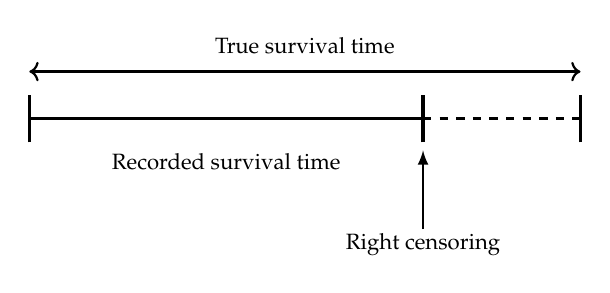
\begin{tikzpicture}
\draw [very thick]  (0,0) -- (5,0) node [below,font=\footnotesize] at (2.5,-0.3) {Recorded survival time};
\draw [very thick] (0,-.3) -- (0, .3);
\draw [very thick] (5,-.3) -- (5, .3);
\draw [very thick, dashed] (5,0) -- (7,0);
\draw [very thick] (7,-.3) -- (7, .3);
\draw [<->,thick] (0,0.6) -- (7,0.6) node [above,font=\footnotesize] at (3.5,0.7) {True survival time};
\node[draw=none, font=\footnotesize] at (5,-1.6) {Right censoring};
\draw[->,>=latex, thick] (5,-1.4) -- (5,-0.4);
\end{tikzpicture}
\end{figure}

Censoring means we do not know the actual survival time.
\end{frame}



\begin{frame}{Right censoring (hypothetical)}

\begin{figure}
\centering
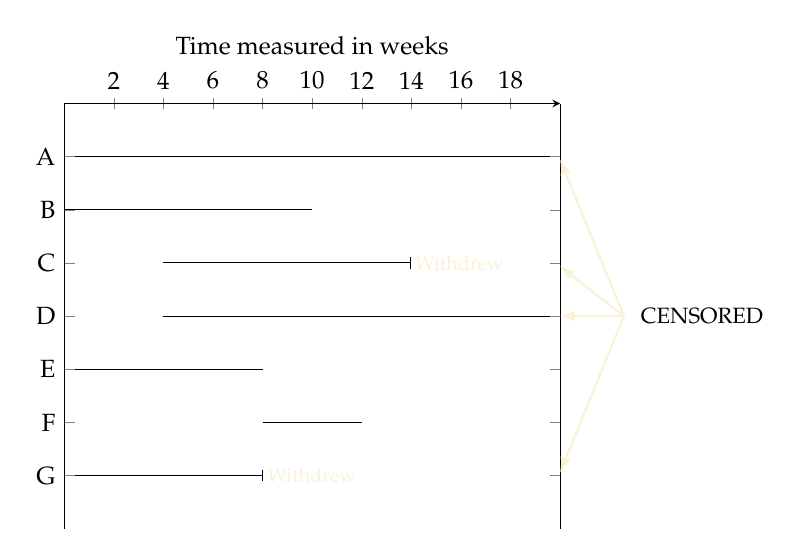
\begin{tikzpicture}[scale=0.9]
 \begin{axis}[smooth,
    area style,
    width=7cm, height=6cm,xmin=0,xmax=5,ymin=0,ymax=2,
    no markers,
    samples=50,
%    axis y line=left,
    axis x line=top,
    scale only axis,
    ytick={0,0.5,1},
%    ylabel={$S(t)$},
%    ylabel style={rotate=-90},
    xtick={0.5,1,1.5,2,2.5,3,3.5,4,4.5},
    xticklabels={2,4,6,8,10,12,14,16,18},
    xlabel={Time measured in weeks},
    ytick={1.75,1.5,1.25,1,0.75,0.5,0.25},
    yticklabels={A,B,C,D,E,F,G}
  ]
  \addplot [thin] coordinates {(0,1.75) (5,1.75)};
  \addplot [thin] coordinates {(0,1.5) (2.5,1.5)} node [right,fore,pos=0.95] {$\bigstar$};
  \addplot [-|,thin] coordinates {(1,1.25) (3.5,1.25)} node [right,fore,pos=0.98, font=\footnotesize] {Withdrew};
  \addplot [thin] coordinates {(1,1) (5,1)};
  \addplot [thin] coordinates {(0,0.75) (2,0.75)} node [right,fore,pos=0.92] {$\bigstar$};
  \addplot [thin] coordinates {(2,0.5) (3,0.5)} node [right,fore,pos=0.87] {$\bigstar$};
  \addplot [-|,thin] coordinates {(0,0.25) (2,0.25)} node [right,fore,pos=0.98, font=\footnotesize] {Withdrew};
  \end{axis}
  \node[draw=none, font=\footnotesize] at (9,3) {CENSORED};
  \draw[->,>=latex,thick,fore] (7.9,3) -- (7,5.2);
  \draw[->,>=latex,thick,fore] (7.9,3) -- (7,3.7);
  \draw[->,>=latex,thick,fore] (7.9,3) -- (7,3);
  \draw[->,>=latex,thick,fore] (7.9,3) -- (7,0.8);
\end{tikzpicture}
\caption*{Study ended on the 20\textsuperscript{th} week. $\bigstar$ denotes event happened.}
\end{figure}

\end{frame}




\begin{frame}{Censoring in my data}



\begin{figure}
\centering
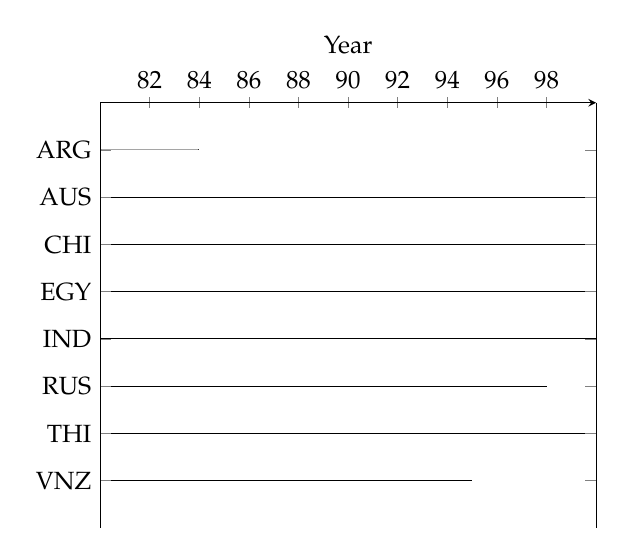
\begin{tikzpicture}[scale=0.9]
 \begin{axis}[smooth,
    area style,
    width=7cm, height=6cm,xmin=0,xmax=5,ymin=0,ymax=2.25,
    no markers,
    samples=50,
%    axis y line=left,
    axis x line=top,
    scale only axis,
    ytick={0,0.5,1},
%    ylabel={$S(t)$},
%    ylabel style={rotate=-90},
    xtick={0.5,1,1.5,2,2.5,3,3.5,4,4.5},
    xticklabels={82,84,86,88,90,92,94,96,98},
    xlabel={Year},
    ytick={2,1.75,1.5,1.25,1,0.75,0.5,0.25},
    yticklabels={ARG,AUS,CHI,EGY,IND,RUS,THI,VNZ}
  ]
  \addplot [thin] coordinates {(0,2) (1,2)} node [right,fore,pos=0.86] {$\bigstar$};
  \addplot [thin] coordinates {(0,1.75) (5,1.75)};
  \addplot [thin] coordinates {(0,1.5) (5,1.5)};
  \addplot [thin] coordinates {(0,1.25) (5,1.25)};
  \addplot [thin] coordinates {(0,1) (5,1)};
  \addplot [thin] coordinates {(0,0.75) (4.5,0.75)} node [right,fore,pos=0.95] {$\bigstar$};
  \addplot [thin] coordinates {(0,0.5) (5,0.5)};
  \addplot [thin] coordinates {(0,0.25) (3.75,0.25)} node [right,fore,pos=0.95] {$\bigstar$};
  \end{axis}
\end{tikzpicture}
\caption*{Study period: 1980--2000. $\bigstar$ denotes event happened.}
\end{figure}

\end{frame}



\begin{frame}{Censoring}
There are other types of censoring as well, although these are less commonly encountered in the social sciences.\bigskip

\textbf{Left censoring}: the actual time is shorter than the one observed by us.\bigskip

\begin{figure}
\centering
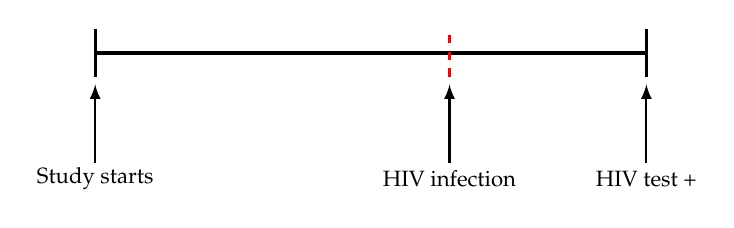
\begin{tikzpicture}
\draw [very thick]  (0,0) -- (7,0);
\node[draw=none, font=\footnotesize] at (7,-1.6) {HIV test +};
\draw[->,>=latex, thick] (7,-1.4) -- (7,-0.4);
\draw [very thick] (0,-.3) -- (0, .3);
\draw [very thick] (7,-.3) -- (7, .3);
\draw [very thick, dashed, color=red] (4.5,-0.3) -- (4.5,0.3);
\node[draw=none, font=\footnotesize] at (4.5,-1.6) {HIV infection};
\draw[->,>=latex, thick] (4.5,-1.4) -- (4.5,-0.4);
\node[draw=none, font=\footnotesize] at (0,-1.6) {Study starts};
\draw[->,>=latex, thick] (0,-1.4) -- (0,-0.4);
\end{tikzpicture}
\end{figure}
\end{frame}



\begin{frame}{Censoring}
\textbf{Interval censoring}: we have a guess as to the bounds of the actual time.\bigskip

\begin{figure}
\centering
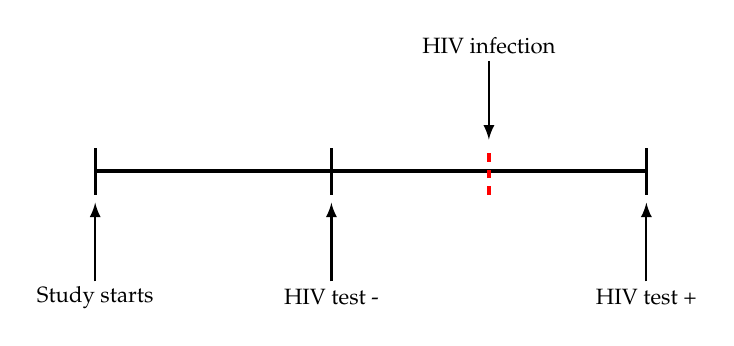
\begin{tikzpicture}
\draw [very thick]  (0,0) -- (7,0);
\node[draw=none, font=\footnotesize] at (3,-1.6) {HIV test -};
\draw[->,>=latex, thick] (3,-1.4) -- (3,-0.4);
\draw [very thick] (3,-.3) -- (3, .3);
\node[draw=none, font=\footnotesize] at (7,-1.6) {HIV test +};
\draw[->,>=latex, thick] (7,-1.4) -- (7,-0.4);
\draw [very thick] (0,-.3) -- (0, .3);
\draw [very thick] (7,-.3) -- (7, .3);
\draw [very thick, dashed, color=red] (5,-0.3) -- (5,0.3);
\node[draw=none, font=\footnotesize] at (5,1.6) {HIV infection};
\draw[->,>=latex, thick] (5,1.4) -- (5,0.4);
\node[draw=none, font=\footnotesize] at (0,-1.6) {Study starts};
\draw[->,>=latex, thick] (0,-1.4) -- (0,-0.4);
\end{tikzpicture}
\end{figure}

Most practical applications of survival analysis deal only with instances of right censoring.
\end{frame}



\subsection{Survivor function}
\begin{frame}{Survivor function}
A survivor function, $S(t)$, gives us the probability that a random observation will survive (not experience the event) past time $t$.\bigskip

To present this in a more intuitive way I grouped my data for 35 of the 70 countries in 3-year periods.\bigskip

With a 7-period division, we have 8 time points to evaluate: 1980, 1983, 1986, 1989, 1992, 1995, 1998, and 2001.


\end{frame}

\begin{frame}{Survivor function}

\begin{table}
\centering
\begin{tabular}{l c c l}
\toprule
Time & Crisis & Total crisis & $S(t)$ \\
\midrule
t=1980 & 0 & 0 & $35/35=1$ \\
t=1983 & 5 & 5 & $30/35=0.8571$ \\
t=1986 & 3 & 8 & $27/35=0.7714$ \\
t=1989 & 2 & 10 & $25/35=0.7143$ \\
t=1992 & 0 & 10 & $25/35=0.7143$ \\
t=1995 & 1 & 11 & $24/35=0.6857$ \\
t=1998 & 3 & 14 & $21/35=0.6$ \\
t=2001 & 2 & 16 & $19/35=0.5429$ \\
\bottomrule
\end{tabular}
\caption*{Survivor function for sovereign debt crises}
\end{table}

``Crises'' denotes number of defaults in $[t-1,t)$ interval, while ``Total crises'' refers to crises in the $[0,t)$ interval.
\end{frame}



\begin{frame}{Survivor function}
We can imagine that if we could let the study run to $\infty$, then the probability of survival would be 0.\bigskip

$S(t)$ uses the information in the ``Total crises'' column. In this sense, it is an actual probability, since it will always range between 0 and 1.\bigskip

At each time point, it uses \textit{all} the information before it to give us the probability that the event will not happen to the remaining observations.
\end{frame}




\begin{frame}{Survivor function}

\begin{figure}
\centering
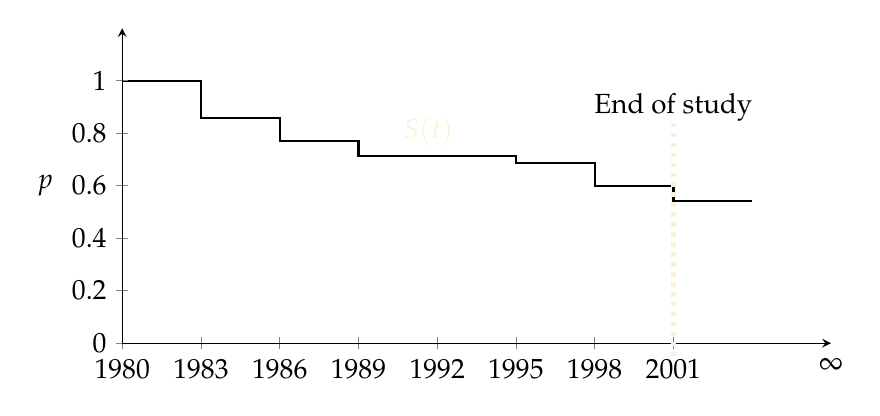
\begin{tikzpicture}
 \begin{axis}[smooth,
    area style,
    width=9cm, height=4cm,xmin=0,xmax=4.5,ymin=0,ymax=1.2,
    no markers,
    samples=50,
    axis y line=left,
    axis x line=bottom,
    scale only axis,
    ytick={0,0.2,0.4,0.6,0.8,1},
    yticklabels={0,0.2,0.4,0.6,0.8,1},
    ylabel={$p$},
    ylabel style={rotate=-90},
    xtick={0, 0.5, 1, 1.5, 2, 2.5, 3, 3.5, 4.5},
    xticklabels={1980, 1983, 1986, 1989, 1992, 1995, 1998, 2001, $\infty$}
  ]
\addplot [const plot, no marks, thick] coordinates {(0,1) (0.5,1) (0.5,0.8571) (1,0.8571) (1,0.7714) (1.5,0.7714) (1.5,0.7143) (2,0.7143) (2.5,0.7143) (2.5,0.6857) (3,0.6857) (3,0.6) (3.5,0.6) (3.5, 0.5429) (4,0.5429)} node[above,pos=0.5,fore] {$S(t)$};]
  \end{axis}
\draw[dotted, ultra thick, fore] (7,2.8) -- (7,-0.2);
\node[draw=none] at (7, 3) {End of study};
\end{tikzpicture}
\caption*{Survivor (step) function for sovereign debt crisis}
\end{figure}

$S(t)$ can also be thought as the proportion of units that survive past time \textit{t}.
\end{frame}




\subsection{Hazard function}
\begin{frame}{Hazard function}
In a sense, the hazard function conveys the opposite information to the survivor function: the probability of the event \textit{happening} per unit of time.\bigskip

This is a \textit{conditional} probability: probability of the event given that it hasn't happened prior to time $t$.\footnote{For now, because we are in the case of discrete periods, I will use the word ``probability''. As we move from the discrete to the continuous world, we will see that we're no longer working with probabilities, but with \textit{rates} (which can be larger than 1).}
\end{frame}




\begin{frame}{Hazard function}

\begin{table}
\centering
\begin{tabular}{l c c l}
\toprule
Time & Crisis & Remaining obs. & $h(t)$ \\
\midrule
t=1980 & 0 & 35 & $0/35=0$ \\
t=1983 & 5 & 35 & $5/35=0.1429$ \\
t=1986 & 3 & 30 & $3/30=0.10$ \\
t=1989 & 2 & 27 & $2/27=0.0741$ \\
t=1992 & 0 & 25 & $0/25=0$ \\
t=1995 & 1 & 25 & $1/25=0.04$ \\
t=1998 & 3 & 24 & $3/24=0.125$ \\
t=2001 & 2 & 21 & $2/21=0.0952$ \\
\midrule
TOTAL & \multicolumn{3}{c}{16} \\
\bottomrule
\end{tabular}
\caption*{Hazard function for sovereign debt crises}
\end{table}
\end{frame}



\begin{frame}{Hazard function}
 The ``Remaining obs.'' column is called the \textit{risk set} -- it quantifies the number of observations which are still at risk to experience the event.\bigskip

Unlike the survival probability, which could only decrease, the hazard probability (rate) can fluctuate from period to period in any direction.\bigskip

\begin{quote}
[\dots] a hazard function $h(t)$ gives the instantaneous potential at time $t$ for getting an event, like death or some disease of interest, given survival up to time $t$. \cite{Kleinbaum2012}
\end{quote}
\end{frame}



\begin{frame}{Hazard vs. survival}

\begin{figure}
\centering
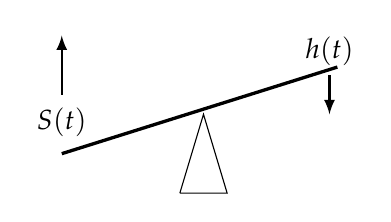
\begin{tikzpicture}
\draw (0,0) -- (0.6,0) -- (0.3,1) -- (0,0);
\draw [very thick] (-1.5,0.5) -- (2,1.6);
\node[draw=none,fill=none] at ++(-1.5,0.9) {$S(t)$};
\draw[->,>=latex, thick] (-1.5,1.25)--(-1.5,2);
\node[draw=none,fill=none] at ++(1.9,1.8) {$h(t)$};
\draw[->,>=latex, thick] (1.9,1.5)--(1.9,1);
\end{tikzpicture}
\end{figure}

The two functions are connected. If the hazard rate is high, the survivor function will be low.
\end{frame}



\begin{frame}{Hazard vs. survival}
\begin{equation}
\centering
h(t)=\frac{f(t)}{S(t)}
\end{equation}

$f(t)$ represents the density function of the survival times.\bigskip

\begin{equation}
\centering
f(t)=\lim_{\Delta t \to 0}\frac{Pr(t \leq T \leq t+\Delta t)}{\Delta t}
\end{equation}

$f(t)$ is the ``\textit{instantaneous} probability an event will occur (or a unit will fail) in the infinitesimally small area bounded by $t$ and $t+\Delta t$.'' \cite[p.~13]{BoxSteffensmeier2004}
\end{frame}



\begin{frame}{Continuous case}

\begin{figure}
\centering
\begin{tikzpicture}
 \begin{axis}[smooth,
    area style,
    width=7cm, height=4cm,xmin=0,xmax=5,ymin=0,ymax=1.2,
    no markers,
    samples=50,
    axis y line=left,
    axis x line=bottom,
    scale only axis,
    ytick={0,1},
%    ylabel={$S(t)$},
%    ylabel style={rotate=-90},
    xtick={2.5, 5},
    xticklabels={$t$,$\infty$}
  ]
\addplot [very thick] coordinates {(0,1) (1,0.95) (2,0.65) (3,0.25) (5,0.05)} node[above,fore,pos=0.50, xshift=0.25cm] {$S(t)$};
  \end{axis}
\end{tikzpicture}
\end{figure}

When time is continuous, these functions themselves are continuous. The formulas become a bit more complex, but the principles remain unchanged.
\end{frame}


\section{Descriptive survival analysis}

\begin{frame}
\begin{center}
\huge Descriptive survival analysis
\end{center}
\end{frame}



\begin{frame}{Comparing survival times}

\begin{figure}
\centering
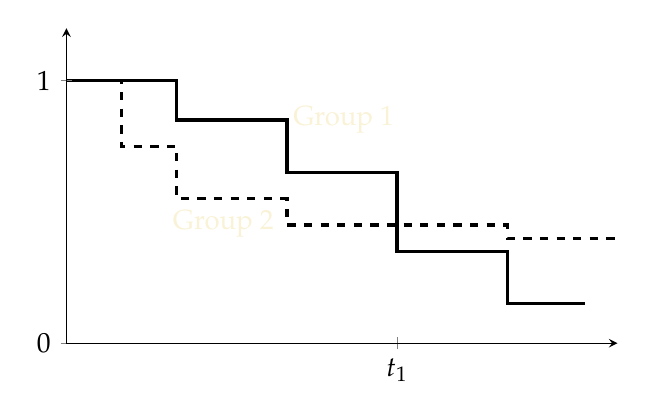
\begin{tikzpicture}
 \begin{axis}[smooth,
    area style,
    width=7cm, height=4cm,xmin=0,xmax=5,ymin=0,ymax=1.2,
    no markers,
    samples=50,
    axis y line=left,
    axis x line=bottom,
    scale only axis,
    ytick={0,1},
%    ylabel={$S(t)$},
%    ylabel style={rotate=-90},
    xtick={3},
    xticklabels={$t_1$}
  ]
\addplot [const plot, no marks, very thick] coordinates {(0,1) (1,1) (1,0.85) (2,0.85) (2,0.65) (3,0.65) (3,0.35) (4,0.35) (4, 0.15) (4.7,0.15)} node[right,pos=0.38,fore] {Group 1};
\addplot [const plot, no marks, very thick, dashed] coordinates {(0,1) (0.5,1) (0.5,0.75) (1,0.75) (1,0.55) (1.5,0.55) (2,0.45) (4,0.45) (4,0.40) (5,0.40)} node[below,pos=0.34,fore] {Group 2};
  \end{axis}
\end{tikzpicture}
\end{figure}

There is clearly a difference between survival times before time $t_1$ and after this moment.
\end{frame}



\begin{frame}{Comparing survival times}

\begin{figure}
\centering
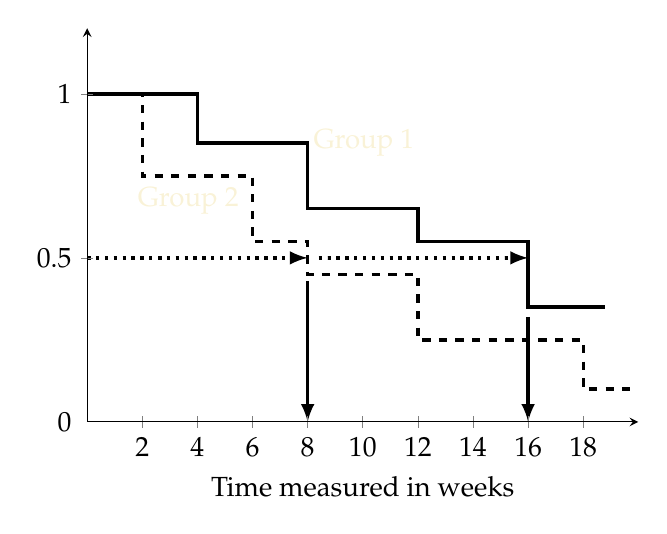
\begin{tikzpicture}
 \begin{axis}[smooth,
    area style,
    width=7cm, height=5cm,xmin=0,xmax=5,ymin=0,ymax=1.2,
    no markers,
    samples=50,
    axis y line=left,
    axis x line=bottom,
    scale only axis,
    ytick={0,0.5,1},
%    ylabel={$S(t)$},
%    ylabel style={rotate=-90},
    xtick={0.5,1,1.5,2,2.5,3,3.5,4,4.5},
    xticklabels={2,4,6,8,10,12,14,16,18},
    xlabel={Time measured in weeks}
  ]
\addplot [const plot, no marks, very thick] coordinates {(0,1) (1,1) (1,0.85) (2,0.85) (2,0.65) (3,0.65) (3,0.55) (4,0.55) (4, 0.35) (4.7,0.35)} node[right,pos=0.38,fore,xshift=0.1cm] {Group 1};
\addplot [const plot, no marks, very thick, dashed] coordinates {(0,1) (0.5,1) (0.5,0.75) (1.5,0.75) (1.5,0.55) (1.5,0.55) (2,0.45) (3,0.45) (3,0.25) (4.5,0.25) (4.5,0.10) (5,0.10)} node[below,pos=0.25,fore, xshift=-0.4cm] {Group 2};
\addplot [->, >=latex, very thick, dotted] coordinates {(0,0.5) (2,0.5)};
\addplot [->, >=latex, very thick] coordinates {(2,0.43) (2,0)};
\addplot [->, >=latex, very thick, dotted] coordinates {(2.1,0.5) (4,0.5)};
\addplot [->, >=latex, very thick] coordinates {(4,0.32) (4,0)};
  \end{axis}
\end{tikzpicture}
\end{figure}

Finding out the median survival time is not difficult at all. Clearly, the first group is doing considerably better than the second one.
\end{frame}




\begin{frame}{Examining data}
In a sense, I'm not treating the data fairly, because Argentina had multiple sovereign debt crises in the 1980s.\bigskip

There are survival analysis techniques that allow you to study multiple occurrence, but they're not covered here.\bigskip

In the 21 years tracked, Argentina was in a debt crisis in 3 years (two separate occasions), Russia in 2 years (one episode), and Venezuela in 4 years (1 episode).
\end{frame}

\begin{frame}{Examining data}
How does the survival duration look for the entire sample?



\begin{figure}
\centering
\includegraphics[scale=0.5]{../03-graphs/01-01}
\caption*{53 out of 70 countries are censored in my data}
\end{figure}
\end{frame}

\subsection{\texttt{survival} package}
\begin{frame}{The \texttt{survival} package}
The most capable and established R package for conducting survival analysis is... \texttt{survival}.\footnote{Created by Thomas Lumley, also the author of the \texttt{survey} package.}\bigskip

\texttt{Zelig} will soon have the capability of running these models (e.g., Cox proportional hazard) but it's too focused on regression for our purposes.\bigskip

For the entire range of descriptive and inferential procedures, we'll use \texttt{survival}.
\end{frame}


\subsection{Kaplan--Meier Survival Curves}
\begin{frame}{Kaplan--Meier}
\begin{equation}
\centering
S(t_{(f)})=\frac{n_{surviving\; past\; t}}{n_{sample}}
\end{equation}

At each point in time, we can compute this quantity, exactly as we did in one of the previous tables.\bigskip

In my example $S(1989)=\frac{25}{35}=0.7143$
\end{frame}

\begin{frame}{Kaplan--Meier}
Alternatively, it can also be computed as a product for individual period probabilities (these are essentially $1 - h(t)$).

\begin{equation}
\centering
S(t)=\prod_{i=1}^t\frac{n_{surviving\; past\; i}}{n_{surviving\; past\; i-1}}
\end{equation}

In my example $S(1989)=\frac{30}{35} \times \frac{27}{30} \times \frac{25}{27}=\frac{25}{35}= 0.7143$\bigskip

These two ways of computing the KM estimate will produce the same result.
\end{frame}

\begin{frame}[fragile]{Survival curves}



\begin{knitrout}\scriptsize
\definecolor{shadecolor}{rgb}{0.988, 0.961, 0.922}\color{fgcolor}\begin{kframe}
\begin{alltt}
\hlkwd{library}\hlstd{(survival)}
\hlcom{# First we have to define a "survival" object, which is then}
\hlcom{# used by the package's functions.}
\hlkwd{Surv}\hlstd{(df_fin}\hlopt{$}\hlstd{time, df_fin}\hlopt{$}\hlstd{event,} \hlkwc{type} \hlstd{=} \hlstr{"right"}\hlstd{)}
\end{alltt}
\begin{verbatim}
 [1] 19+ 12   2  19+  2   6  19+ 19+ 19+ 19   1  19+  2  19+ 19+ 19+ 17  19+ 19+
[20] 19+  2   4   5  19+  8  19+  5  19+ 19+ 18  16  19+ 19+ 15  19+
\end{verbatim}
\begin{alltt}
\hlcom{# The "type" argument asks what kind of censoring we have in}
\hlcom{# our data, with 6 options. "right" is the default, but I}
\hlcom{# added it here nonetheless. Other common options are "left"}
\hlcom{# or "interval".}
\end{alltt}
\end{kframe}
\end{knitrout}

Right censored observations are marked with a \texttt{+} in the output.
\end{frame}




\begin{frame}[fragile]{Estimating KM curves}

\begin{knitrout}\scriptsize
\definecolor{shadecolor}{rgb}{0.988, 0.961, 0.922}\color{fgcolor}\begin{kframe}
\begin{alltt}
\hlstd{ObjSurv1} \hlkwb{<-} \hlkwd{survfit}\hlstd{(}\hlkwd{Surv}\hlstd{(time, event)} \hlopt{~} \hlnum{1}\hlstd{,} \hlkwc{data} \hlstd{= df_fin)}
\hlcom{# ~1 means that the entire sample is used for 1 KM curve.}
\end{alltt}
\end{kframe}
\end{knitrout}

The \texttt{survfit()} function will do the actual estimation of the Kaplan-Meier survival curves.\bigskip

\begin{knitrout}\scriptsize
\definecolor{shadecolor}{rgb}{0.988, 0.961, 0.922}\color{fgcolor}\begin{kframe}
\begin{alltt}
\hlkwd{round}\hlstd{(}\hlkwd{summary}\hlstd{(ObjSurv1)}\hlopt{$}\hlstd{surv,} \hlkwc{digits} \hlstd{=} \hlnum{2}\hlstd{)}
\end{alltt}
\begin{verbatim}
 [1] 0.97 0.86 0.83 0.77 0.74 0.71 0.69 0.66 0.63 0.60 0.57 0.54
\end{verbatim}
\end{kframe}
\end{knitrout}

Lower and \textbf{upper} confidence bounds for these estimates are also produced and easily accessible.\bigskip

\begin{knitrout}\scriptsize
\definecolor{shadecolor}{rgb}{0.988, 0.961, 0.922}\color{fgcolor}\begin{kframe}
\begin{alltt}
\hlkwd{round}\hlstd{(}\hlkwd{summary}\hlstd{(ObjSurv1)}\hlopt{$}\hlstd{upper,} \hlkwc{digits} \hlstd{=} \hlnum{2}\hlstd{)}
\end{alltt}
\begin{verbatim}
 [1] 1.00 0.98 0.96 0.92 0.90 0.88 0.86 0.83 0.81 0.79 0.76 0.74
\end{verbatim}
\end{kframe}
\end{knitrout}

\end{frame}



\begin{frame}[fragile]{Estimating KM curves}



\begin{knitrout}\scriptsize
\definecolor{shadecolor}{rgb}{0.988, 0.961, 0.922}\color{fgcolor}\begin{kframe}
\begin{alltt}
\hlkwd{plot}\hlstd{(ObjSurv1,} \hlkwc{xlab} \hlstd{=} \hlstr{"Time"}\hlstd{,} \hlkwc{ylab} \hlstd{=} \hlstr{"Survival probability"}\hlstd{)}
\end{alltt}
\end{kframe}
\end{knitrout}

\begin{figure}[ht]
  \centering
  \includegraphics[width=0.7\textwidth]{../03-graphs/01-02.pdf}
\end{figure}
\end{frame}



\begin{frame}[fragile]{Estimating KM curves}

\begin{knitrout}\scriptsize
\definecolor{shadecolor}{rgb}{0.988, 0.961, 0.922}\color{fgcolor}\begin{kframe}
\begin{alltt}
\hlkwd{rm}\hlstd{(ObjSurv1)}
\hlstd{ObjSurv2} \hlkwb{<-} \hlkwd{survfit}\hlstd{(}\hlkwd{Surv}\hlstd{(time, event)} \hlopt{~} \hlstd{SouthA,} \hlkwc{data} \hlstd{= df_fin)}
\hlcom{# Compute separate curves for two groups. The formula can}
\hlcom{# accommodate numerous situations, involving multiple}
\hlcom{# group membership indicators.}
\end{alltt}
\end{kframe}
\end{knitrout}

The same command for plotting can be used in this instance as well.\bigskip



\begin{knitrout}\scriptsize
\definecolor{shadecolor}{rgb}{0.988, 0.961, 0.922}\color{fgcolor}\begin{kframe}
\begin{alltt}
\hlkwd{plot}\hlstd{(ObjSurv2,} \hlkwc{xlab} \hlstd{=} \hlstr{"Time"}\hlstd{,} \hlkwc{ylab} \hlstd{=} \hlstr{"Survival probability"}\hlstd{,}
     \hlkwc{conf.int} \hlstd{=} \hlnum{TRUE}\hlstd{)}
\hlcom{# The defaults with more than two groups is not to plot CIs.}
\hlcom{# Here, though, I've asked it to plot them. When there is}
\hlcom{# only one group, however, CIs are plotted by default.}
\end{alltt}
\end{kframe}
\end{knitrout}

\end{frame}




\begin{frame}[fragile]{Estimating KM curves}

\begin{figure}[ht]
  \centering
  \includegraphics[width=0.6\textwidth]{../03-graphs/01-03.pdf}
\end{figure}

Should we be content with these bland graphics? I think we shouldn't.
\end{frame}



\begin{frame}[fragile]{Estimating KM curves}




\begin{knitrout}\scriptsize
\definecolor{shadecolor}{rgb}{0.988, 0.961, 0.984}\color{fgcolor}\begin{kframe}
\begin{alltt}
\hlstd{ObjSurvMod2} \hlkwb{<-} \hlkwd{createSurvivalFrame}\hlstd{(ObjSurv2)}
\hlkwd{rm}\hlstd{(ObjSurv2)}
\hlkwd{qplot_survival}\hlstd{(ObjSurvMod2)} \hlopt{+} \hlkwd{xlab}\hlstd{(}\hlstr{"Time"}\hlstd{)} \hlopt{+} \hlkwd{ylab}\hlstd{(}\hlstr{"Survival"}\hlstd{)}
\end{alltt}
\end{kframe}
\end{knitrout}



The functions \texttt{createSurvivalFrame()} and \texttt{qplot\_survival()} were created by Ramon Saccilotto.\bigskip

You can modify these yourselves, for better control of the graph (e.g. line thickness, proper legend), or just extract the quantities manually and use them in \texttt{ggplot2}.\footnote{Watch out for the \texttt{ggfortify} package, which will probably be launched soon on CRAN.}
\end{frame}




\begin{frame}[fragile]{Estimating KM curves}

\begin{figure}[ht]
  \centering
  \includegraphics[width=0.6\textwidth]{../03-graphs/01-04.pdf}
\end{figure}

By default, the functions plot the KM survival estimates without confidence intervals, as in the standard \texttt{plot()} function.
\end{frame}



\begin{frame}[fragile]{Estimating KM curves}

\begin{knitrout}\scriptsize
\definecolor{shadecolor}{rgb}{0.988, 0.961, 0.922}\color{fgcolor}\begin{kframe}
\begin{alltt}
\hlkwd{qplot_survival}\hlstd{(ObjSurvMod2,} \hlnum{TRUE}\hlstd{)} \hlopt{+} \hlkwd{xlab}\hlstd{(}\hlstr{"Time"}\hlstd{)} \hlopt{+}
    \hlkwd{ylab}\hlstd{(}\hlstr{"Survival"}\hlstd{)}
\end{alltt}
\end{kframe}
\end{knitrout}



\begin{figure}[ht]
  \centering
  \includegraphics[width=0.6\textwidth]{../03-graphs/01-05.pdf}
\end{figure}

\end{frame}



\subsection{Log-rank test}

\begin{frame}{Log-rank test}

How do we truly know that the two curves are different from each other, when taking into account the uncertainty around them?\bigskip

The \texttt{log-rank test} can be used for this.\bigskip

It is essentially a $\chi^2$ test, which relies on observed vs. expected\footnote{What would be expected if the null hypothesis of no effect would be true.} cell counts in the different outcome categories.

\end{frame}



\begin{frame}{Log-rank: theoretical}
Assume we have a particular point in time, which we denote as $t$, and the two groups we're trying to compare, which I'll label as $A$ and $B$.\bigskip

The expected cell count for group $A$ at time $t$ is, in this situation:

\begin{equation}
\centering
e_A=\frac{n_{risk\; A}}{n_{risk\; A} + n_{risk\; B}} \times (n_{fail\; A} + n_{fail\; B})
\end{equation}

The first term in the equation is the proportion of elements in the risk set, which gets multiplied with the total number of events.
\end{frame}




\begin{frame}{Log-rank: theoretical}
Identically, the expected cell count at time $t$ for group $B$ is:

\begin{equation}
\centering
e_B=\frac{n_{risk\; B}}{n_{risk\; A} + n_{risk\; B}} \times (n_{fail\; A} + n_{fail\; B})
\end{equation}

For each group, we can compute the sum of the difference between observed and expected cell counts at each time point. For example, for $A$,\bigskip

\begin{equation}
\centering
O_A - E_A = \sum_{1}^{n_{fail\; A}}(n_{fail\; A} - e_A)
\end{equation}
\end{frame}




\begin{frame}{Log-rank: theoretical}
Finally, the log-rank test statistic value for any one of the two groups is

\begin{equation}
\centering
Log-rank = \frac{(O_A - E_A)^2}{Var(O_A - E_A)}
\end{equation}

\begin{equation}
\centering
\scriptsize
Var(O_A-E_A)=\frac{n_{risk\; A} \times n_{risk\; B} \times (n_{fail\; A}+n_{fail\; B}) \times (n_{risk\; A}+n_{risk\; B} - n_{fail\; A} - n_{fail\; B})}{(n_{risk\; A}+n_{risk\; B})^2(n_{risk\; A}+n_{risk\; B}-1)}
\end{equation}

\end{frame}




\begin{frame}{Log-rank: practical}
This will have a $\chi^2$ distribution with 1 degree of freedom (in the situation when we're comparing only 2 groups).\footnote{When comparing N groups, it will be N-1 degrees of freedom.}\bigskip

I tried doing all these calculations by hand, but I must have made a mistake somewhere because I got a slightly different result at the decimal points.\bigskip

So I switched to a pre-worked example, on a different data set.
\end{frame}



\begin{frame}{Log-rank: practical}

\begin{figure}
\centering
\includegraphics[height=0.8\textheight]{../03-graphs/01-08.png}
\hspace{0.33cm}
\includegraphics[height=0.8\textheight]{../03-graphs/01-09.png}
\end{figure}
\end{frame}


\begin{frame}{Log-rank: practical}

\begin{figure}
\centering
\includegraphics[width=0.6\textwidth]{../03-graphs/01-06.png}
\caption*{From \citeA[p.~69]{Kleinbaum2012}.}
\end{figure}

\end{frame}



\begin{frame}{Log-rank: practical}

\begin{figure}
\centering
\includegraphics[width=0.6\textwidth]{../03-graphs/01-07.png}
\caption*{From \citeA[p.~71]{Kleinbaum2012}.}
\end{figure}

But how would this test work in my case?
\end{frame}



\begin{frame}[fragile]{Log-rank: practical}

\begin{knitrout}\scriptsize
\definecolor{shadecolor}{rgb}{0.988, 0.961, 0.922}\color{fgcolor}\begin{kframe}
\begin{alltt}
\hlkwd{survdiff}\hlstd{(}\hlkwd{Surv}\hlstd{(time, event)} \hlopt{~} \hlstd{SouthA,} \hlkwc{data} \hlstd{= df_fin)}
\end{alltt}
\begin{verbatim}
Call:
survdiff(formula = Surv(time, event) ~ SouthA, data = df_fin)

          N Observed Expected (O-E)^2/E (O-E)^2/V
SouthA=0 27       10    12.99     0.689      3.82
SouthA=1  8        6     3.01     2.973      3.82

 Chisq= 3.8  on 1 degrees of freedom, p= 0.05 
\end{verbatim}
\end{kframe}
\end{knitrout}

It's technically not statistically significant. It's anyone's guess, but my personal opinion is that with a slightly larger sample size for one of the groups, we could have found a significant difference.
\end{frame}




\begin{frame}{Log-rank: theoretical}
For more groups, the formulas get considerably more complicated, but the software cares little about this.\bigskip

However, there are numerous variants of the log-rank test, which differ in how they weight the time points.\bigskip

As you could see from the formula, Kaplan--Meier weights each point equally when computing the final test statistic.
\end{frame}




\begin{frame}{Log-rank: theoretical}

\begin{table}
\centering
\begin{tabular}{l l}
\toprule
Test statistic & $w(t)$ \\
\midrule
Log-rank & 1 \\
Wilcoxon & $n_{risk}$ \\
Tarone-Ware & $\sqrt{n_{risk}}$ \\ 
Peto & $\widetilde{s}(t)$ \\
Flemington-Harrington\footnote{Offers maximum flexibility because the user supplies the values for $p$ and $q$.} & $\widehat{S}(t)^p \times [1 - \widehat{S}(t)]^q$ \\
\bottomrule
\end{tabular}
\end{table}

There might be valid situations when you want to assign more influence to earlier time points, e.g. if you believe that a drug would have a more dramatic short-term effect than a long-term one.
\end{frame}




\begin{frame}[fragile]{Log-rank: theoretical}

Only the Peto variant is implemented in the \texttt{survival} package.\bigskip

\begin{knitrout}\scriptsize
\definecolor{shadecolor}{rgb}{0.988, 0.961, 0.922}\color{fgcolor}\begin{kframe}
\begin{alltt}
\hlkwd{survdiff}\hlstd{(}\hlkwd{Surv}\hlstd{(time, event)} \hlopt{~} \hlstd{SouthA,} \hlkwc{data} \hlstd{= df_fin,} \hlkwc{rho} \hlstd{=} \hlnum{1}\hlstd{)}
\end{alltt}
\begin{verbatim}
Call:
survdiff(formula = Surv(time, event) ~ SouthA, data = df_fin, 
    rho = 1)

          N Observed Expected (O-E)^2/E (O-E)^2/V
SouthA=0 27     7.97    10.29     0.521      3.34
SouthA=1  8     4.80     2.49     2.155      3.34

 Chisq= 3.3  on 1 degrees of freedom, p= 0.07 
\end{verbatim}
\end{kframe}
\end{knitrout}

The Wilcoxon test is available in the \texttt{stats} package, the Flemington--Harrington in \texttt{FHtest}, and the Tarone--Ware in \texttt{EnvStats}.


\end{frame}



\section{Conclusion}

\begin{frame}{Conclusion}
We had to go through these terms because they are quite unique to the entire modeling approach.\bigskip

So far we've mainly been concerned with the descriptive part of survival analysis. We also made small steps into the inferential area.\bigskip

Tomorrow we go full-inferential with the Cox proportional-hazards model.
\end{frame}


\begin{frame}
\begin{center}
    \Huge Thank \textcolor{title}{you} for the kind attention!
\end{center}
\end{frame}

% REFERENCES %

\begin{frame}{References}
\bibliographystyle{apacite}
\bibliography{../Bibliography}
\end{frame}

\end{document}
